\documentclass[12pt]{article} % 12pt 为字号大小 UTF8
\usepackage{amssymb,amsfonts,amsmath,amsthm}
%\usepackage{fontspec,xltxtra,xunicode}
%\usepackage{times}

%----------
% 定义中文环境
%----------

\usepackage{xeCJK}

% \setCJKmainfont[BoldFont={SimHei},ItalicFont={KaiTi}]{SimSun}
% \setCJKsansfont{SimHei}
% \setCJKfamilyfont{zhsong}{SimSun}
% \setCJKfamilyfont{zhhei}{SimHei}

% \newcommand*{\songti}{\CJKfamily{zhsong}} % 宋体
% \newcommand*{\heiti}{\CJKfamily{zhhei}}   % 黑体


%----------
% 版面设置
%----------
%首段缩进
\usepackage{indentfirst}
\setlength{\parindent}{2.1em}

%行距
\renewcommand{\baselinestretch}{1.4} % 1.4倍行距

%页边距
\usepackage[a4paper]{geometry}
\geometry{verbose,
	tmargin=3cm,% 上边距
	bmargin=3cm,% 下边距
	lmargin=3cm,% 左边距
	rmargin=3cm % 右边距
}


%----------
% 其他宏包
\usepackage{listings}

%----------
%图形相关
\usepackage[x11names]{xcolor} % must before tikz, x11names defines RoyalBlue3
\usepackage{graphicx}
\usepackage{pstricks,pst-plot,pst-eps}
\usepackage{subfig}
\def\pgfsysdriver{pgfsys-dvipdfmx.def} % put before tikz
\usepackage{tikz}

%原文照排
\usepackage{verbatim}

%网址
\usepackage{url}
\usepackage[framed,numbered,autolinebreaks,useliterate]{mcode}

%----------
% 习题与解答环境
%----------
% %习题环境
% \theoremstyle{definition} 
% \newtheorem{exs}{习题}

% %解答环境
% \ifx\proof\undefined\
% \newenvironment{proof}[1][\protect\proofname]{\par
% \normalfont\topsep6\p@\@plus6\p@\relax
% \trivlist
% \itemindent\parindent
% \item[\hskip\labelsep
% \scshape
% #1]\ignorespaces
% }{%
% \endtrivlist\@endpefalse
% }
% \fi

% \renewcommand{\proofname}{\it{证明}}

%----------
% 我的自定义
%----------

\newcommand{\horrule}[1]{\rule[0.5ex]{\linewidth}{#1}} 	% Horizontal rule

\renewcommand{\refname}{参考文献}
\renewcommand{\abstractname}{\large \bf 摘\quad 要}
\renewcommand{\contentsname}{目录}
\renewcommand{\tablename}{表}
\renewcommand{\figurename}{图}

\setlength{\parskip}{0.4ex} % 段落间距

\usepackage{enumitem}
\setenumerate[1]{itemsep=0pt,partopsep=0pt,parsep=\parskip,topsep=5pt}
\setitemize[1]{itemsep=0.4ex,partopsep=0.4ex,parsep=\parskip,topsep=0.4ex}
\setdescription{itemsep=0pt,partopsep=0pt,parsep=\parskip,topsep=5pt}


%==========
% 正文部分
%==========

\begin{document}
	
	\title{
	%	{\normalfont\normalsize\textsc{
	%			Xiangtan University  \\[25pt]}}
		\horrule{0.5pt}\\
		\sffamily{数值计算方法实验报告\\矩阵的LU分解}
		\horrule{1.8pt}\\[20pt]
	}
	\author{米科润\quad 19信计二班\\201905755824}
	\date{\today} % 若不需要自动插入日期,则去掉前面的注释;{ } 中也可以自定义日期格式
	
	\begin{titlepage}
		\maketitle
		\vspace{30pt}
		\thispagestyle{empty}
	\end{titlepage}
	
	\tableofcontents
	\thispagestyle{empty}
	
	\newpage
	\setcounter{page}{1}
	
	\section{实验题目}
	随机生成一个 $5\times5$ 的矩阵,其中每个元素为属于[11,24]的整数,矩阵不能为对称矩阵,做LU分解(各阶顺序主子式不能为0)
	
	
	\section{实现算法}
	对随机生成的非对称非奇异矩阵
	\begin{center}
	$A=
	\begin{bmatrix}
		a_{11} &\cdots& a_{1n} \\
		\vdots &\ddots& \vdots \\
		a_{n1} &\cdots& a_{nn}
	\end{bmatrix}$
	\end{center}
	\indent 利用Gauss顺序消去法:将A分解为$A=L\cdot U$,其中
	\begin{center}
	$L=
	\begin{bmatrix}
		1  \\
		l_{21}   &1& \\
		\vdots  &&  &\ddots& \\
		l_{n1} &\cdots& &l_{n,n-1}& &1&
	\end{bmatrix}$,
	$U=
	\begin{bmatrix}
		u_{11} &u_{12}& &\cdots& &u_{1n}& \\
		0 &u_{22}& &\cdots& &u_{2n}& \\
		\vdots &\ddots& &\ddots& &\vdots& \\
		0 &\cdots& &0& &u_{nn}&
	\end{bmatrix}$
	\end{center}
	\indent U为A进行行变换生成的上三角矩阵(主对角元素不为0),而L的每一个元素为对应行变换的系数的相反数。
	
	
	
	\section{程序代码}
	编写Gauss顺序消去法函数并保存为Gauss.m
	\begin{lstlisting}
	function [] = Gauss(A)
	%A=randi([11,24],5);生成的随机矩阵
	%L为生成的下三角矩阵,U为生成的上三角矩阵
	n=size(A,1);L=eye(n);
	%%
	%判断A的各阶顺序主子式是否奇异
	%for k = 1:n
	%    if det(A(1:k,1:k)) == 0
	%        error('A的顺序主子式有奇异');
	%    end
	%end
	%%
	%判断A是否为奇异矩阵
	if det(A) == 0
	error('A为奇异矩阵,请输入非奇异矩阵');
	end
	%%
	%判断A是否为对称阵
	if A==A'
	error('A为对称阵');
	end
	%%
	%LU分解
	for i =2:n
		if A(i-1,i-1) == 0%做行变换使对角线元素不为0
			for j = i:n
				if A(j,j) ~= 0
					A([i-1,j],:) = A([j,i-1],:);
					break
				end
			end
		end
		m = A(i:n,i-1)./A(i-1,i-1);
		L(i:n,i-1)=m;
		A(i:n,:) = A(i:n,:) - m*A(i-1,:);
	end
	U=A;
	%%
	%输出信息
	disp('L为:');disp(L);
	disp('U为:');disp(U);
	end
	\end{lstlisting}

	\section{实验结果}
	在命令窗口输入:\\
	$>>$A=randi([11,24],5)\\
	$>>$Gauss(A)\\
	\indent 回车可得运算结果:
	\begin{figure}[ht]
		\centering
		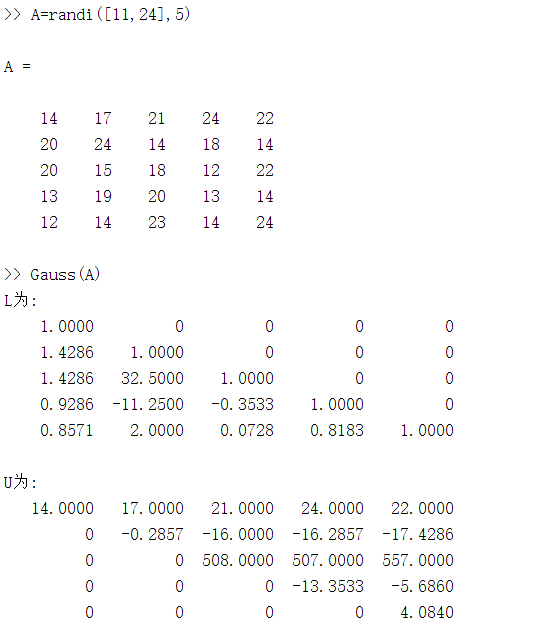
\includegraphics[width=0.95\textwidth]{Gauss.png}
		\caption{result}
		\label{fig:fig1}
	\end{figure}
	% \section{习题环境}
	
	% \begin{exs}
	% 请证明勾股定理。
	% \end{exs}
	% \begin{proof}
	% 这是证明。末尾后会自动添加方块以示结束。
	% \end{proof}
	
	% \begin{exs}
	% 请计算 $1+2+\ldots +100$。
	% \end{exs}
	% \begin{proof}[解答]
	% 这是解答。末尾后会自动添加方块以示结束。
	% \end{proof}
	
	
\end{document}